\documentclass[11pt,a4paper,oneside,english,italian]{book} 

\usepackage[a4paper]{geometry}
\geometry{verbose, tmargin=4cm, bmargin=4cm, lmargin=3cm, rmargin=3cm, headsep=0.5cm, footskip=1cm}

\usepackage[italian]{babel}

% Pacchetto necessario ad impostare l'interlinea
\usepackage{setspace}

% Package impiegato per editare e formattare opportunamente frammenti di pseudocodice.
\usepackage{algorithmic}

% algorithm serve per incapsulare algorithmic al fine di ottenere un oggetto flotable come una figura o una tabella.
\usepackage{algorithm}

% Pacchetto graphicx per inserire figure in LaTeX. Maggiori dettagli sull'utilizzo del pacchetto sono riportati di seguito.
\usepackage{graphicx} 
\graphicspath{{./figure/}}


% Questi pacchetti consentono di centrare il contenuto di una tabella
\usepackage{multirow}
\usepackage{comment}
\usepackage{array}
\newcolumntype{P}[1]{>{\centering\arraybackslash}p{#1}}
\newcolumntype{M}[1]{>{\centering\arraybackslash}m{#1}}
\newcolumntype{L}[1]{>{\arraybackslash}m{#1}}
\usepackage{xcolor,colortbl}
\usepackage{tabularray}
\definecolor{red}{rgb}{1,0,0}

% Metadati
\usepackage{hyperref}  
\hypersetup{
    pdftitle={Progetto di Sistemi Cyberfisici di Mattia Marino},
    pdfauthor={Mattia Marino}
}

% Matematica
\usepackage{amsmath, amsfonts, amssymb, amsthm}

% Indentazione automatica anche nel primo paragrafo
\usepackage{indentfirst}

% Redifinizione della riga di testa delle pagine:
\usepackage{fancyhdr}
\pagestyle{fancy}

\renewcommand{\chaptermark}[1]{\markboth{#1}{}}
\renewcommand{\sectionmark}[1]{\markright{\thesection\ #1}}
\fancyhf{}
\fancyhead[LO]{\bfseries\rightmark}
\renewcommand{\headrulewidth}{0.5pt}
\renewcommand{\footrulewidth}{0.5pt}
\setlength{\headheight}{14.5pt}

% Pacchetti addizionali per inserire più tabelle o figure fianco a fianco
\usepackage{caption}
\usepackage{subcaption}
\usepackage{booktabs}
\usepackage{float}         
	

% Da qui inizia il documento, fino ad ora si è preparato il preambolo
\begin{document}

% Titolo
\frontmatter

% Frontespizio e dedica
\linespread{1} % per il frontespizio utilizzo l'interlinea singola

\thispagestyle{empty}
\large

% % % % % % % % % % % % % % % % % % % % 
% TESTO IN CORSIVO
% % \emph{\textbf{UNIVERSITA' DEGLI STUDI DEL SANNIO}}\\
% % \textbf{\emph{Facolt?  di Ingegneria}}\\
% % \textbf{\emph{Corso di Laurea Specialistica in \\Ingegneria delle
		% % Telecomunicazioni}}
% % % % % % % % % % % % % % % % % % 

% INTESTAZIONE DEL FRONTESPIZIO
\begin{center}
	\huge{{\underline{\textsc{UNIVERSIT\`A DEGLI STUDI DEL SANNIO}}}}
\end{center}

\begin{center}   
	\huge{{\textsc{DIPARTIMENTO DI INGEGNERIA}}}
	\\
	\LARGE{\textbf{\\Corso di Laurea Magistrale in \\Ingegneria Informatica}}      
	
\end{center}

%******************************************************************
%                                   Logo Unisannio
%******************************************************************
\begin{figure}[h]
	\begin{center}
		
\includegraphics[scale=0.3]{figure/logo/logoUniSannio_new.jpg}
	\end{center}
\end{figure}
%******************************************************************                                

\vspace{0.25cm}

%
%
% TITOLO DELLA TESI
\begin{center}
    Analisi e Controllo di Sistemi Cyberfisici
    
	{\LARGE \textbf{PROGETTAZIONE DI UN SEMAFORO A CORSIA MULTIPLA ORIENTATO AL PARALLELISMO} \smallskip\\}                                               
\end{center}

% RELATORE E CANDIDATO DELLA TESI
\vspace{2cm}
\begin{tabular}{ll}
	\textit{Prof.ssa:}        \hspace{3cm}   	& \textit{Autore:}\\
	\textbf{Elisa Mostacciuolo}      \hspace{5cm}     & \textbf{Mattia Marino}\\   
	\hspace{3cm}      & \textit{Matr:399000634}                                       					   
	%                        
\end{tabular}

% ANNO ACCADEMICO     
\vspace{2.5cm}
\begin{center}
	\textsc{Anno Accademico 2024/2025}
\end{center}

% Nuova pagina    
\newpage


% Numerazione delle prime pagine in numeri romani
\pagenumbering{roman}

% Set del conunter al valore 1, questo evita che vengono conteggiate anche la pagine del frontespizio, facendo partire il conteggio da 3 piuttosto che da 1
\setcounter{page}{0}

% Indice della tesi
\tableofcontents

% Rispristino il valore dell'interlinea a 1.5, quadunque nel frontespizio venisse posto ad 1.0
\onehalfspacing

% Introduzione
\chapter*{Introduzione}
\label{cap:introduzione}

\addcontentsline{toc}{chapter}{Introduzione}
\lhead{\bfseries INTRODUZIONE}
\rhead{\thepage}

Nel contesto tecnologico attuale, i Cyber-Physical Systems (CPS) stanno acquisendo un'importanza sempre maggiore. Questi sistemi integrati, che combinano componenti fisici con capacità computazionali, hanno trasformato vari settori, dall'industria alla sanità, dai trasporti all'energia. Tipicamente, ciò avviene attraverso loop di feedback in cui i processi fisici influenzano la computazione e viceversa. Affinché il sistema possa rispondere ai cambiamenti esterni e correggere il proprio comportamento, è essenziale che la parte fisica e quella computazionale comunichino tramite una rete. I CPS possono impiegare sensori, attuatori, elettronica e software avanzato che collaborano per monitorare, controllare e ottimizzare sistemi reali in tempo reale. Questa interazione tra il mondo cibernetico e quello fisico offre numerosi vantaggi, tra cui maggiore efficienza operativa, sicurezza migliorata, riduzione dei costi e ottimizzazione delle risorse (che nei sistemi embedded sono spesso molto limitate). Questo documento descrive e dettaglia il lavoro svolto nella progettazione e modellazione di un CPS per il controllo di un sistema di semafori stradali in un'intersezione stradale con un focus particolare sul parallelismo dei veicoli che attraversano l'incrocio, qualora possibile.
\chapter*{Problem Statement}
\label{cap:problem-statement}

\addcontentsline{toc}{chapter}{Problem Statement}
\lhead{\bfseries PROBLEM STATEMENT}
\rhead{\thepage}

Il progetto ivi trattato si pone l'obiettivo di progettare e modellare il comportamento di un insieme di semafori stradali in un'intersezione. In particolare, si è scelto di riprogettare un semaforo già esistente, con lo scopo di migliorarne l'efficienza e la sicurezza. Il semaforo scelto a tale scopo è quello presente all'incrocio tra Via del Pomerio, Ponte Vanvitelli, Via Posillipo e Corso Vittorio Emanuele III, a Benevento. Al fine di spiegare meglio la dinamica dell'intersezione, si riportano due schermate catturate da Google Maps, che mostrano l'incrocio in questione (Fig. \ref{fig:intersection_top} e Fig. \ref{fig:intersection_3d}).

\begin{figure}[H]
    \centering
    \begin{minipage}[b]{.45\textwidth}
        \centering
        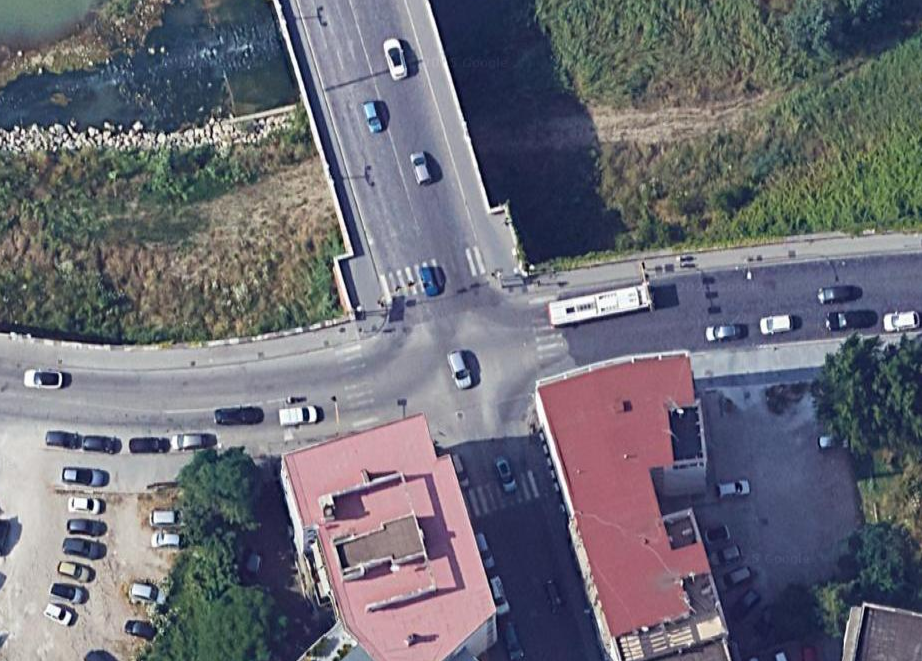
\includegraphics[width=\textwidth]{figure/intersection/incrocio_top.png}
        \caption{Vista dall'alto dell'intersezione}
        \label{fig:intersection_top}
    \end{minipage}
    \hfill
    \begin{minipage}[b]{.45\textwidth}
        \centering
        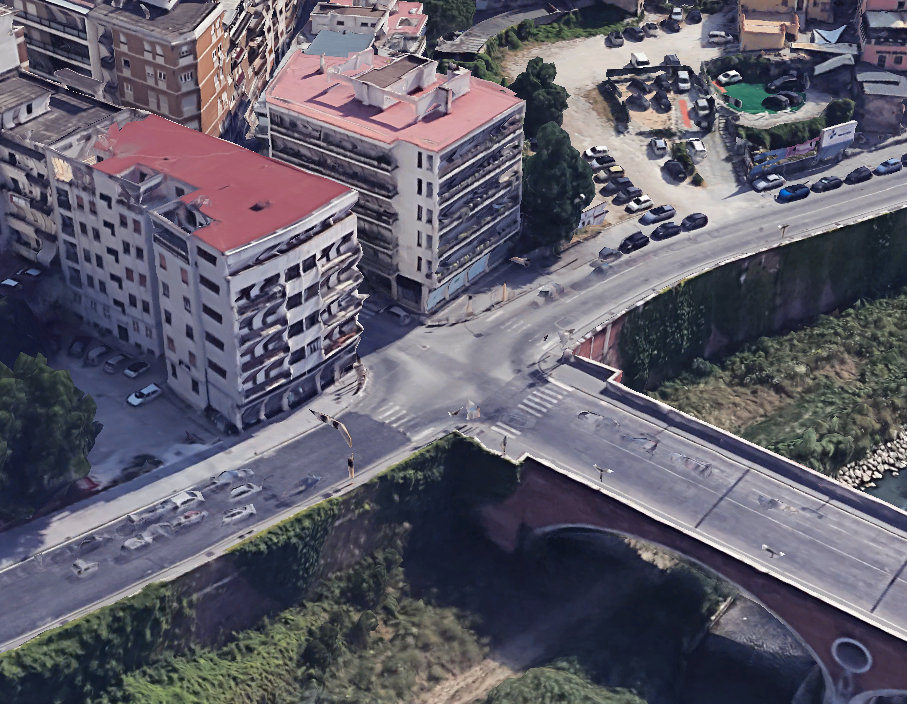
\includegraphics[width=\textwidth]{figure/intersection/incrocio_3d.png}
        \caption{Vista 3D dell'intersezione}
        \label{fig:intersection_3d}
    \end{minipage}
\end{figure}

Come si può quindi dedurre dall'immagine, a Est si trovano tre semafori che consentono di andare a Nord, Sud e Ovest. A Ovest, invece, si trovano due semafori che consentono di andare a Nord e a Sud. Il semaforo a Nord, infine, consente di andare a Ovest o a Sud. Ogni combinazione provenienza-destinazione si trova su un'apposita corsia e ha un semaforo dedicato.

Al fine di modellare il comportamento del semaforo, si è scelto di utilizzare il formalismo delle Reti di Petri, in quanto permette di modellare sistemi concorrenti e distribuiti in modo chiaro e intuitivo. Nel caso modellato, per migliorare l'efficienza del semaforo, si è scelto di permettere il passaggio di più veicoli contemporaneamente, qualora possibile, imponendo vincoli per evitare che due o più veicoli si incrocino. Ad esempio è consentito il passaggio contemporaneo di un veicolo proveniente da Est diretto verso Nord e uno proveniente da Ovest e diretto verso Sud. Al contrario, invece, non è possibile attraversare contemporaneamente l'incrocio con due veicoli provenienti da direzioni diverse e diretti nella stessa direzione, in quanto ciò potrebbe causare un incidente. Inoltre, non è possibile che due veicoli si incontrino all'interno dell'incrocio, come ad esempio un veicolo che attraversa l'incrocio da Est a Ovest e un veicolo che attraversa l'incrocio da Nord a Sud.

Tali vincoli sono stati modellati con l'utilizzo di GMEC, come mostrato nelle sezioni successive.

% Corpo del documento
\mainmatter
\chapter{Reti di Petri}
\label{cap:cap1}
\lhead{\textbf{\rightmark}}
In questo capitolo viene discussa la teoria che si trova alla base 
della Rete di Petri utilizzata per modellare questo progetto. Si parte 
dal dare una definizione generale, per poi andare più nel dettaglio 
spiegando i concetti di matrice di pre e post incidenza, marcatura, e GMEC.
\newpage

\section{Definizione}
\label{sec:1.1}
Una Rete di Petri è un formalismo matematico per la modellazione di sistemi distribuiti discreti. In termini più semplici, è un modo per descrivere come funzionano i sistemi in cui accadono eventi discreti e concorrenti, ovvero eventi che possono accadere in parallelo. Immagina un sistema con diverse attività che possono svolgersi contemporaneamente o in sequenza, con risorse che vengono utilizzate e rilasciate: una Rete di Petri fornisce un linguaggio grafico e matematico per rappresentare e analizzare questo tipo di sistemi.

\subsection{Componenti Chiave di una Rete di Petri}
Una Rete di Petri è rappresentata graficamente come un grafo bipartito composto da quattro elementi fondamentali:
\begin{itemize}
    \item \textbf{Posti:} Rappresentati da cerchi, i posti rappresentano le condizioni o gli stati del sistema. Ad esempio, un posto potrebbe rappresentare la disponibilità di una risorsa, lo stato di un processo (attivo, inattivo, in attesa), o una condizione logica (vero/falso).
    \item \textbf{Transizioni:} Rappresentate da rettangoli o barre, le transizioni rappresentano gli eventi o le azioni che possono accadere nel sistema. L'attivazione di una transizione causa un cambiamento nello stato del sistema.
    \item \textbf{Archi:} Rappresentati da frecce dirette, gli archi connettono i posti alle transizioni e le transizioni ai posti, definendo le relazioni di causa-effetto tra stati ed eventi. Un arco che va da un posto a una transizione indica una pre-condizione per l'attivazione della transizione; un arco che va da una transizione a un posto indica un effetto post-attivazione della transizione.
    \item \textbf{Marcatura:} La marcatura di una rete è la distribuzione di token (generalmente rappresentati da punti neri) all'interno dei posti. La marcatura rappresenta lo stato corrente del sistema. Il numero di token in un posto indica quante "unità" di quella condizione sono presenti.
\end{itemize}

\subsection{Funzionamento di una Rete di Petri}
L'evoluzione di una Rete di Petri è regolata da una semplice regola di scatto (firing):
\begin{itemize}
    \item \textbf{Abilitazione:} Una transizione è abilitata (può scattare) se tutti i posti di input (i posti da cui partono archi verso la transizione) contengono almeno un token.
    \item \textbf{Scatto:} Quando una transizione abilitata scatta, vengono rimossi un token da ciascun posto di input e viene aggiunto un token a ciascun posto di output (i posti a cui arrivano archi dalla transizione).
\end{itemize}

Nelle Reti di Petri, l'enfasi è posta sulle regole che governano le transizioni tra i vari stati, piuttosto che sugli stati stessi. Questo approccio rende il modello più versatile e adatto a rappresentare sistemi dinamici e complessi, dove il numero di stati possibili può essere indefinito o teoricamente infinito.

\newpage

\section{Matrici di Pre e Post incidenza}
\label{sec:1.2}
Le matrici di pre e post-incidenza, insieme alla matrice di incidenza, sono strumenti matematici fondamentali per rappresentare e analizzare le Reti di Petri in modo formale. Permettono di descrivere le connessioni tra posti e transizioni e di studiare il comportamento dinamico della rete attraverso calcoli matriciali.

\subsection{Matrice di Pre-incidenza}
La matrice di pre-incidenza, indicata con \textit{Pre}, descrive le connessioni che vanno dai posti alle transizioni. È una matrice \textit{n x m}, dove \textit{n} è il numero di posti e \textit{m} è il numero di transizioni nella rete. L'elemento \textit{Pre(p, t)} della matrice indica il numero di archi che vanno dal posto \textit{p} alla transizione \textit{t}. In altre parole, rappresenta il numero di token che devono essere presenti nel posto p affinché la transizione t sia abilitata a scattare.

\begin{itemize}
    \item Se \textit{Pre(p, t) = 0}, non esiste un arco che connette il posto \textit{p} alla transizione \textit{t}.
    \item Se \textit{Pre(p, t) = 1}, esiste un singolo arco che connette il posto \textit{p} alla transizione \textit{t}.
    \item Se \textit{Pre(p, t) > 1}, esistono più archi (archi multipli) che connettono il posto \textit{p} alla transizione \textit{t}.
\end{itemize}

\subsection{Matrice di Post-incidenza}
La matrice di post-incidenza, indicata con \textit{Post}, descrive le connessioni che vanno dalle transizioni ai posti. È anch'essa una matrice \textit{n x m}, con \textit{n} posti e \textit{m} transizioni. L'elemento \textit{Post(p, t)} indica il numero di archi che vanno dalla transizione \textit{t} al posto \textit{p}. Rappresenta il numero di token che vengono depositati nel posto \textit{p} quando la transizione \textit{t} scatta.

\begin{itemize}
    \item Se \textit{Post(p, t) = 0}, non esiste un arco che connette la transizione \textit{t} al posto \textit{p}.
    \item Se \textit{Post(p, t) = 1}, esiste un singolo arco che connette la transizione \textit{t} al posto \textit{p}.
    \item Se \textit{Post(p, t) > 1}, esistono più archi che connettono la transizione \textit{t} al posto \textit{p}.
\end{itemize}

\subsection{Matrice di Incidenza}
La matrice di incidenza, indicata con \textit{C}, è derivata dalle matrici di pre e post-incidenza e fornisce una rappresentazione compatta delle variazioni di marcatura causate dallo scatto delle transizioni. Essa è definita come:
\begin{equation}
    C = Post - Pre
    \label{eq:incidence_matrix}
\end{equation}

L'elemento \textit{C(p, t)} della matrice di incidenza indica quindi la variazione netta del numero di token nel posto \textit{p} quando la transizione \textit{t} scatta:

\begin{itemize}
    \item Se \textit{C(p, t) > 0}, lo scatto di \textit{t} aggiunge token al posto \textit{p}.
    \item Se \textit{C(p, t) < 0}, lo scatto di \textit{t} rimuove token dal posto \textit{p}.
    \item Se \textit{C(p, t) = 0}, lo scatto di \textit{t} non influenza il numero di token nel posto \textit{p}.
\end{itemize}
\newpage

\section{Marcatura}
\label{sec:1.3}
La marcatura è un altro concetto centrale nelle Reti di Petri, in quanto rappresenta lo stato del sistema modellato in un dato istante. In termini semplici, la marcatura indica la distribuzione dei \textit{token} (generalmente rappresentati da punti neri) all'interno dei \textit{posti} della rete.

Formalmente, una marcatura \textit{M} di una Rete di Petri è una funzione che associa ad ogni posto \textit{p} un numero intero non negativo, \textit{M(p)}. Questo numero rappresenta il numero di token presenti nel posto \textit{p}. Possiamo rappresentare la marcatura come un vettore, dove l'i-esimo elemento del vettore corrisponde al numero di token nel posto i-esimo.

Graficamente, i token sono disegnati all'interno dei cerchi che rappresentano i posti. Se un posto non contiene token, il suo cerchio è vuoto. Se un posto contiene più di un token, il numero di token è solitamente indicato all'interno del cerchio. Generalmente il numero di token in un posto è rappresentato disegnando un cerchio con un numero di punti neri uguale al numero di token presenti, ma in caso in cui tale numero sia elevato è anche possibile scrivere semplicemente il numero.

\subsection{Marcatura Iniziale}
La marcatura iniziale, spesso indicata con \textit{M0}, rappresenta lo stato di partenza del sistema. È la marcatura da cui inizia l'esecuzione della rete. La scelta della marcatura iniziale è cruciale, poiché determina il comportamento che la rete può esibire. Come spiegato nella sezione \ref{sec:1.4} è anche possibile che la marcatura iniziale scelta sia illegale per via dei vincoli imposti dalla rete.

\subsection{Evoluzione della Marcatura}
L'evoluzione di una Rete di Petri è determinata dallo scatto delle transizioni. Lo scatto di una transizione modifica la marcatura della rete secondo le seguenti regole:

\begin{itemize}
    \item \textbf{Abilitazione:} Una transizione \textit{t} è abilitata se ogni posto di input di \textit{t} (cioè ogni posto da cui parte un arco verso \textit{t}) contiene almeno un numero di token pari al peso dell'arco (se non specificato, il peso è 1).
    \item \textbf{Scatto:} Quando una transizione t abilitata scatta: 
    \begin{itemize}
        \item Viene rimosso da ogni posto di input di \textit{t} un numero di token pari al peso dell'arco che lo connette a \textit{t}.
        \item Viene aggiunto a ogni posto di output di \textit{t} (cioè ogni posto a cui arriva un arco da \textit{t}) un numero di token pari al peso dell'arco che lo connette a \textit{t}.
    \end{itemize}
\end{itemize}

Questo processo di scatto delle transizioni causa una transizione da una marcatura all'altra, descrivendo l'evoluzione dinamica del sistema modellato.

\subsection{Raggiungibilità}
Un concetto importante legato alla marcatura è la \textit{raggiungibilità}. Una marcatura \textit{M'} è raggiungibile da una marcatura \textit{M} se esiste una sequenza di scatti di transizioni che, partendo da \textit{M}, porta alla marcatura \textit{M'}. L'insieme di tutte le marcature raggiungibili da una marcatura iniziale \textit{M0} è detto \textit{insieme di raggiungibilità di M0}. L'analisi dell'insieme di raggiungibilità è fondamentale per studiare le proprietà del sistema modellato, come la boundedness (limitazione del numero di token nei posti), la liveness (possibilità di scatto delle transizioni) e la reversibilità (possibilità di tornare alla marcatura iniziale).
\newpage

\section{GMEC}
\label{sec:1.4}
Le Generalized Mutual Exclusion Constraints (GMEC), o Vincoli Generalizzati di Mutua Esclusione, sono un potente formalismo utilizzato nell'analisi e nel controllo delle Reti di Petri, specialmente in contesti dove è necessario garantire che certe combinazioni di marcature non si verifichino mai. In altre parole, le GMEC definiscono insiemi di posti la cui somma di token non deve superare una determinata soglia. Questo è particolarmente utile per modellare risorse condivise, vincoli di capacità, o condizioni di sicurezza in sistemi concorrenti.

Una GMEC è espressa tipicamente come una disuguaglianza lineare sulla marcatura \textit{M} della Rete di Petri:

\begin{equation}
    \sum_{p \in P} w_{p} \cdot M(p) \leq k
\end{equation}

dove:

\begin{itemize}
    \item $P$ è un insieme di posti della rete.
    \item $w_{p}$ è un peso non negativo associato al posto p.
    \item $M(p)$ è il numero di token nel posto p nella marcatura M.
    \item $k$ è una costante intera non negativa che rappresenta la capacità o la soglia massima.
\end{itemize}

Volendo scrivere il tutto in forma vettoriale e definendo il vettore $w$ come il vettore dei pesi associati ai posti, e il vettore $M$ come il vettore delle marcature, possiamo scrivere la disuguaglianza come:

\begin{equation}
    w^{T} \times M \leq k
\end{equation}

\subsection{Posto monitor}
Il concetto di "posto monitor", o "supervisore", è strettamente legato all'implementazione delle GMEC nelle Reti di Petri. L'obiettivo è di trasformare una disuguaglianza (la GMEC) in un'uguaglianza, introducendo un nuovo posto, il posto monitor, che "monitora" il rispetto del vincolo.

Data una GMEC scritta in forma vettoriale:

\begin{equation}
    w^{T} \times M \leq k
\end{equation}

Introduciamo un nuovo posto, che chiameremo $p_{m}$ (posto monitor), che avrà come matrice di incidenza un vettore riga  di lunghezza \textit{n} (dove \textit{n} è il numero di transizioni della rete):

\begin{equation}
    C_{m} = -w^{T} \times C
\end{equation}

Da tale vettore è possibile quindi capire come il posto monitor si colleghi al resto della rete già esistente. Inoltre, per calcolare la marcatura iniziale del posto monitor:

\begin{equation}
    M(p_{m}) = k - w^{T} \times M_{0}
\end{equation}

\subsection{GMEC multiple}
Qualora ci fossero GMEC multiple, come nel caso ivi preso in esame, è possibile calcolare rapidamente le matrici di incidenza dei posti monitor associati a ciascuna GMEC e le relative marcature iniziali utilizzando delle semplici operazioni matriciali.

Considerando quindi un inzieme di GMEC, è possibile esprimere i loro vettori peso come righe di una matrice $W$:

\begin{equation}
    W = \begin{bmatrix}
        w_{1} \\
        w_{2} \\
        \vdots \\
        w_{m}
    \end{bmatrix}
\end{equation}

L'equazione quindi diventa:

\begin{equation}
    C_{m} = -W \times C
    \label{eq:gmec_vect}
\end{equation}

Similmente, esprimendo le costanti $k$ come un vettore colonna $K$, è possibile calcolare le marcature iniziali dei posti monitor come:

\begin{equation}
    M(p_{m}) = K - W \times M_{0}
    \label{eq:gmec_init}
\end{equation}
\newpage


\chapter{PIPE 2}
\label{cap:cap2}
\lhead{\textbf{\rightmark}}
PIPE (Platform Independent Petri Net Editor) è un software progettato per supportare la modellazione, l'analisi e la simulazione delle reti di Petri. Si tratta di uno strumento potente e versatile che offre un'interfaccia intuitiva per rappresentare visivamente sistemi complessi attraverso diagrammi basati sulle reti di Petri. PIPE si distingue per la sua capacità di combinare un approccio grafico user-friendly con strumenti avanzati di analisi e simulazione, rendendolo una scelta ideale per ingegneri, ricercatori e sviluppatori che lavorano su sistemi distribuiti, processi aziendali e reti di comunicazione.

\begin{figure}
    \centering
    \begin{minipage}[b]{.45\textwidth}
        \centering
        
\includegraphics[width=\textwidth]{figure/pipe/pipe_logo.png}
        \caption{Logo di PIPE 2}
        \label{fig:pipe_logo}
    \end{minipage}
    \hfill
    \begin{minipage}[b]{.45\textwidth}
        \centering
        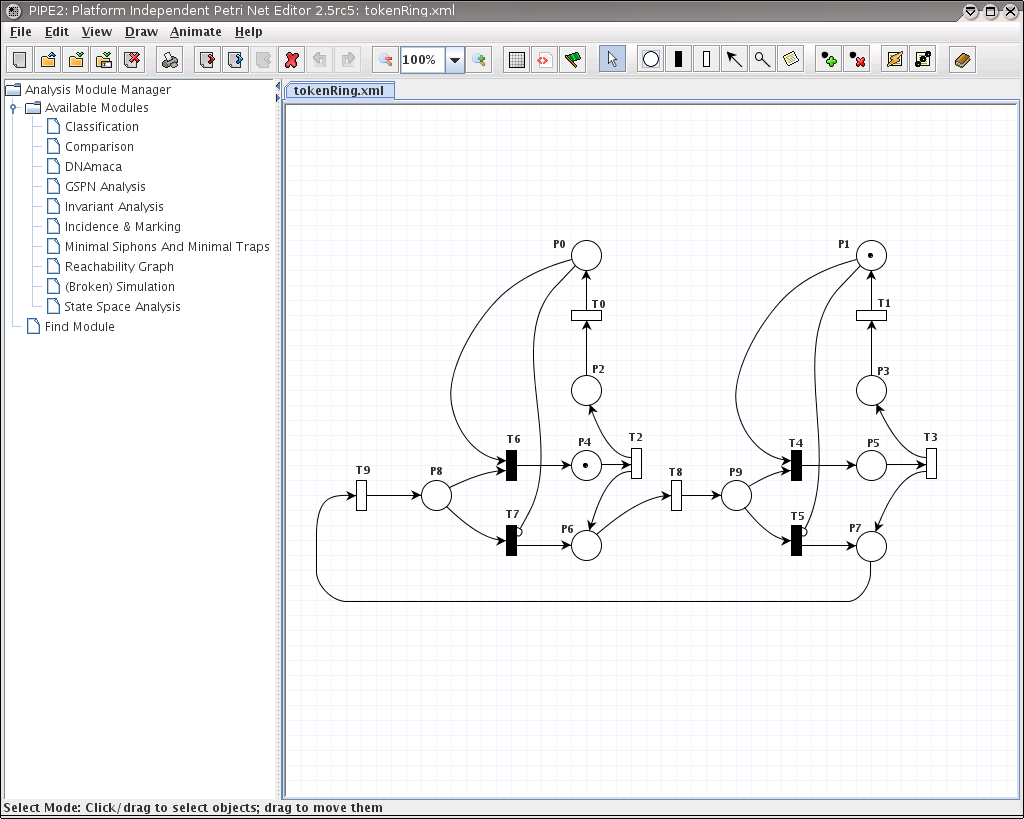
\includegraphics[width=\textwidth]{figure/pipe/pipe_example.png}
        \caption{Esempio di PIPE 2}
        \label{fig:pipe_example}
    \end{minipage}
\end{figure}

\newpage
Segue ora un breve elenco riportante alcune funzionalità di PIPE 2 che ne hanno portato alla scelta come software per la realizzazione di questo progetto.

\begin{itemize}
    \item \textbf{Interfaccia grafica intuitiva}
    PIPE offre un ambiente visuale semplice ma potente che consente agli utenti di progettare reti di Petri in modo interattivo. Gli elementi principali del modello, come posti (posti di memoria o risorse, rappresentati da cerchi), transizioni (eventi o processi, rappresentati da rettangoli) e archi direzionali (che collegano posti e transizioni), possono essere creati e configurati facilmente con pochi clic. Questa semplicità d'uso riduce la curva di apprendimento per i principianti e accelera il lavoro degli esperti.
    
    \item \textbf{Progettazione di reti di Petri}
    Con PIPE è possibile costruire reti di Petri che rappresentano la logica e il flusso di informazioni di un sistema. Grazie al supporto per la modellazione grafica, l'utente può rappresentare visivamente il comportamento del sistema, rendendo più comprensibile la struttura complessiva. Ad esempio, un sistema produttivo può essere rappresentato da posti che indicano le risorse disponibili, transizioni che rappresentano i processi produttivi e archi che mostrano le relazioni tra risorse e processi.
    
    \item \textbf{Proprietà, attributi e personalizzazione}
    Uno degli aspetti distintivi di PIPE è la possibilità di aggiungere attributi dettagliati agli elementi della rete. Ogni arco, posto o transizione può essere personalizzato con proprietà specifiche, come i pesi degli archi, i tempi di ritardo associati alle transizioni o altre caratteristiche peculiari del sistema. Questo consente di creare modelli estremamente accurati, in grado di rappresentare fedelmente la complessità del sistema reale.
    
    \item \textbf{Analisi avanzata e simulazione dinamica}
    PIPE non si limita alla semplice creazione di reti di Petri, ma offre anche potenti strumenti di analisi e simulazione. L'utente può eseguire simulazioni per osservare il comportamento dinamico del sistema nel tempo, identificando colli di bottiglia, verificando proprietà di sicurezza (ad esempio, l'assenza di deadlock) o analizzando il throughput di risorse. Questo permette di testare le prestazioni del sistema in condizioni diverse e di ottenere preziose informazioni per ottimizzarne il design.
\end{itemize}
\newpage


\chapter{Progettazione}
\label{cap:cap3}
\lhead{\textbf{\rightmark}}
La progettazione di questo progetto è stata suddivisa in due parti principali: inizialmente, infatti, c'è stata una fase di ricerca e studio sulle Reti di Petri per rappresentare un semaforo semplice in maniera ottimale e sicura, per poi passare a una fase di progettazione vera e propria del semaforo finale. Inizialmente, quindi, si propone una versione semplificatta del progetto costituita da due semafori che regolano due strade perpendicolari, per poi passare alla versione finale caratterizzante il semaforo presente all'incrocio preso in esame e descritto in precedenza.
\newpage

\section{Approccio semplificato}
\label{sec:3.1}
La versione del semaforo trattata in questa sezione del progetto è una versione semplificata del lavoro finale, volta a spiegare il funzionamento del semaforo come progettato. Tale semaforo, infatti, costituisce l'unità fondamentale di questo lavoro ed è poi ripreso successivamente nel progetto finale.

\begin{figure}[h]
    \centering
    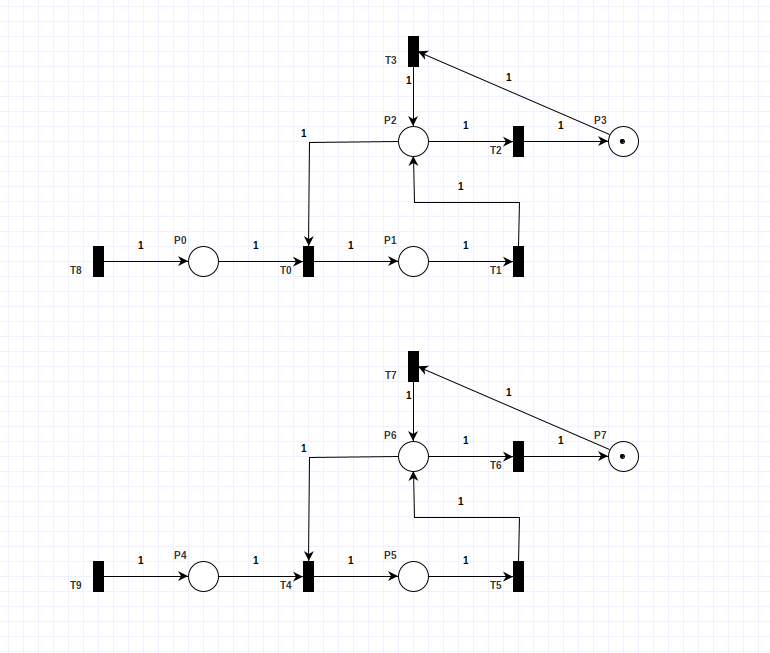
\includegraphics[width=0.6\textwidth]{figure/project_screenshots/semafori.png}
    \caption{Versione base con due semafori}
    \label{fig:semafori}
\end{figure}

In figura \ref{fig:semafori} possiamo vedere una prima bozza di questo progetto. Prendiamo ora in esame solo il semaforo di sopra: il posto P0 rappresenta la fila dei veicoli in attesa di passare, mentre il posto P1 rappresenta un veicolo che attraversa l'incrocio. La transizione T8 a sua volta ha lo scopo di creare un nuovo veicolo da inserire in coda agli altri in P0. I posti P2 e P3, invece, rappresentano una prima struttura di controllo del semaforo: P2 abilita il passaggio, mentre P3 conserva un token bloccando invece il semaforo. Come si può notare, il posto P2 abilita la transizione T0, che permette al veicolo di attraversare l'incrocio. La transizione T1, invece, permette al veicolo di uscire dall'incrocio e di liberare il posto P1 e facendo tornare il token in P2, rendendo il semaforo pronto per un altro attraversamento o per passare al rosso (P3).

Tuttavia, tale versione presenta alcuni importanti difetti che non è possibile ignorare: allo stato attuale i due semafori possono lavorare in maniera indipendente, rendendo possibili scenari pericolosi quali l'attraversamento contemporanreo di due veicoli. A tal scopo. quindi, sono state implementate due GMEC: 

\begin{itemize}
    \item \textbf{GMEC 1}: solo un semaforo alla volta può essere verde:
    \begin{equation}
        M(P_{2}) + M(P_{6}) \leq 1
    \end{equation}

    \item \textbf{GMEC 2}: non è possibile che due veicoli si incrocino:
    \begin{equation}
        M(P_{1}) + M(P_{5}) \leq 1
    \end{equation}
\end{itemize}

\begin{figure}[h]
    \centering
    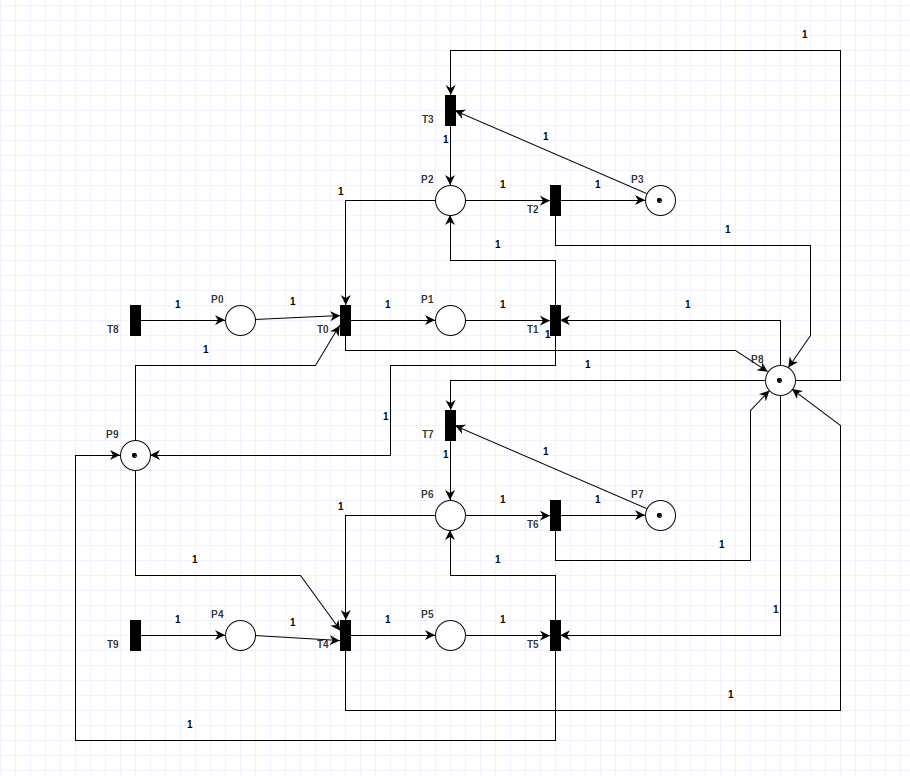
\includegraphics[width=0.6\textwidth]{figure/project_screenshots/semafori_con_controllo.png}
    \caption{Versione con GMEC}
    \label{fig:semafori_gmec}
\end{figure}

Grazie a questi due vincoli, il semaforo diventa come quanto mostrato in figura \ref{fig:semafori_gmec}. In questo modo, quindi, è possibile garantire un attraversamento stradale sicuro e ordinato dell'incrocio.
\newpage

\section{Modello finale}
\label{sec:3.2}
Viene ora presentata, invece, la versione completa e finale del progetto. Anche qui, come nel caso precedente, si inizia con un modello senza posti monitor. Tale modello è presentato in Fig. \ref{fig:semafori_finale}.

\begin{figure}[ht]
    \centering
    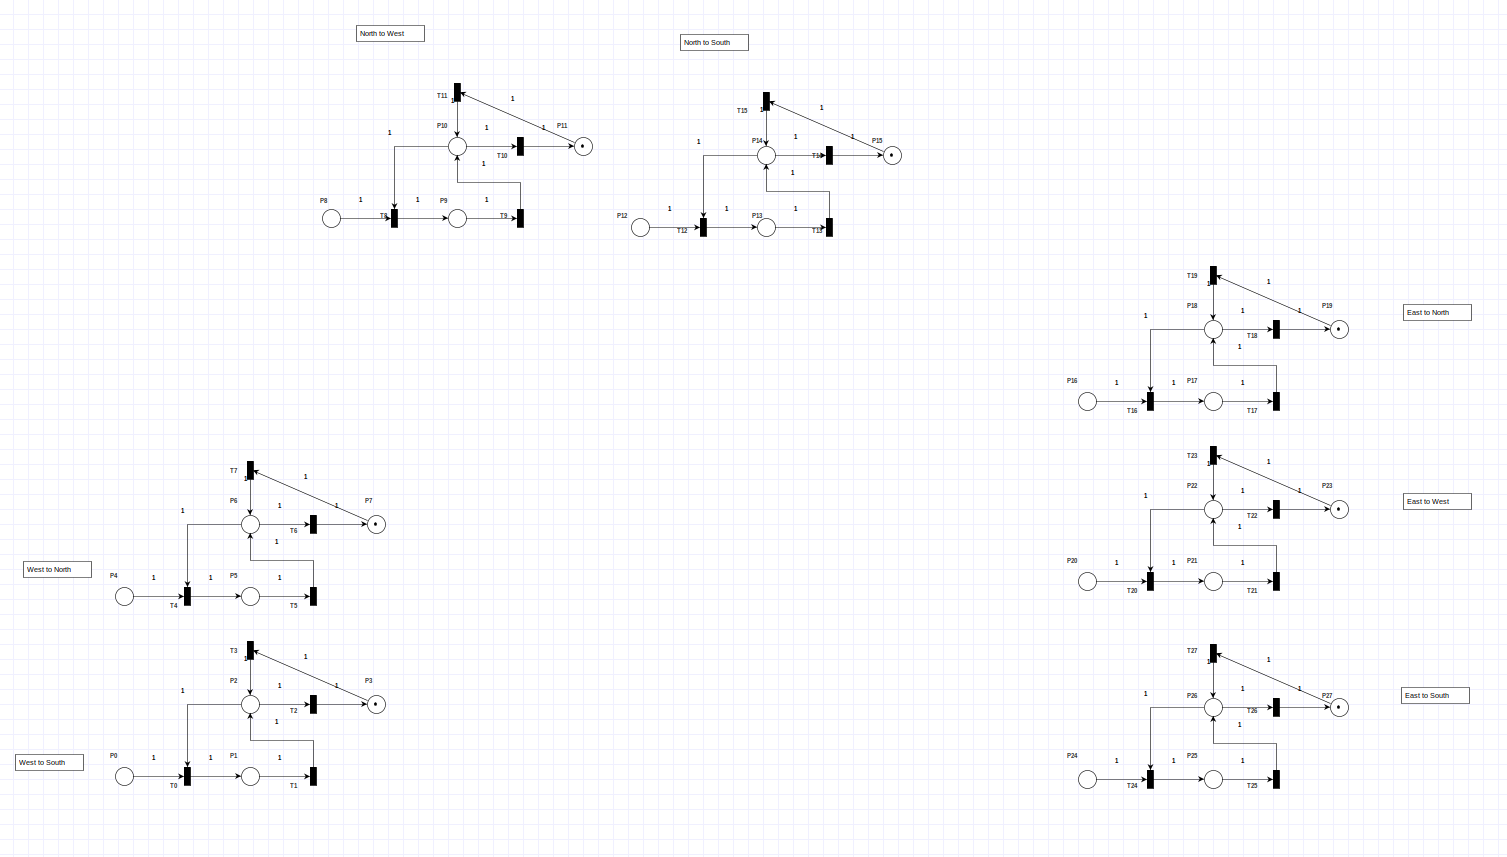
\includegraphics[width=0.8\textwidth]{figure/project_screenshots/semafori_finale.png}
    \caption{Modello finale senza controlli}
    \label{fig:semafori_finale}
\end{figure}

Appare subito evidente, quindi, come questo sia semplicemente una ripetizione del semaforo visto nella sezione \ref{sec:3.1}. Sono state inoltre aggiunte alcune etichette per fare chiarezza sulla direzione di provenienza e di destinazione dei veicoli.

Si procede, dunque, con l'implenentare tutti i vincoli richiesti come dettagliati nella sezione successiva. Il modello finale, con i posti monitor, è presentato in Fig. \ref{fig:semafori_finale_monitor}. Tale modello impedisce che due veicoli si incrocino all'interno dell'incrocio, come ad esempio un veicolo che attraversa l'incrocio da Est a Ovest e un veicolo che attraversa l'incrocio da Nord a Sud. Inoltre, non è possibile attraversare contemporaneamente l'incrocio con due veicoli provenienti da direzioni diverse e diretti nella stessa direzione, in quanto ciò potrebbe causare un incidente.

\begin{figure}[htb]
    \centering
    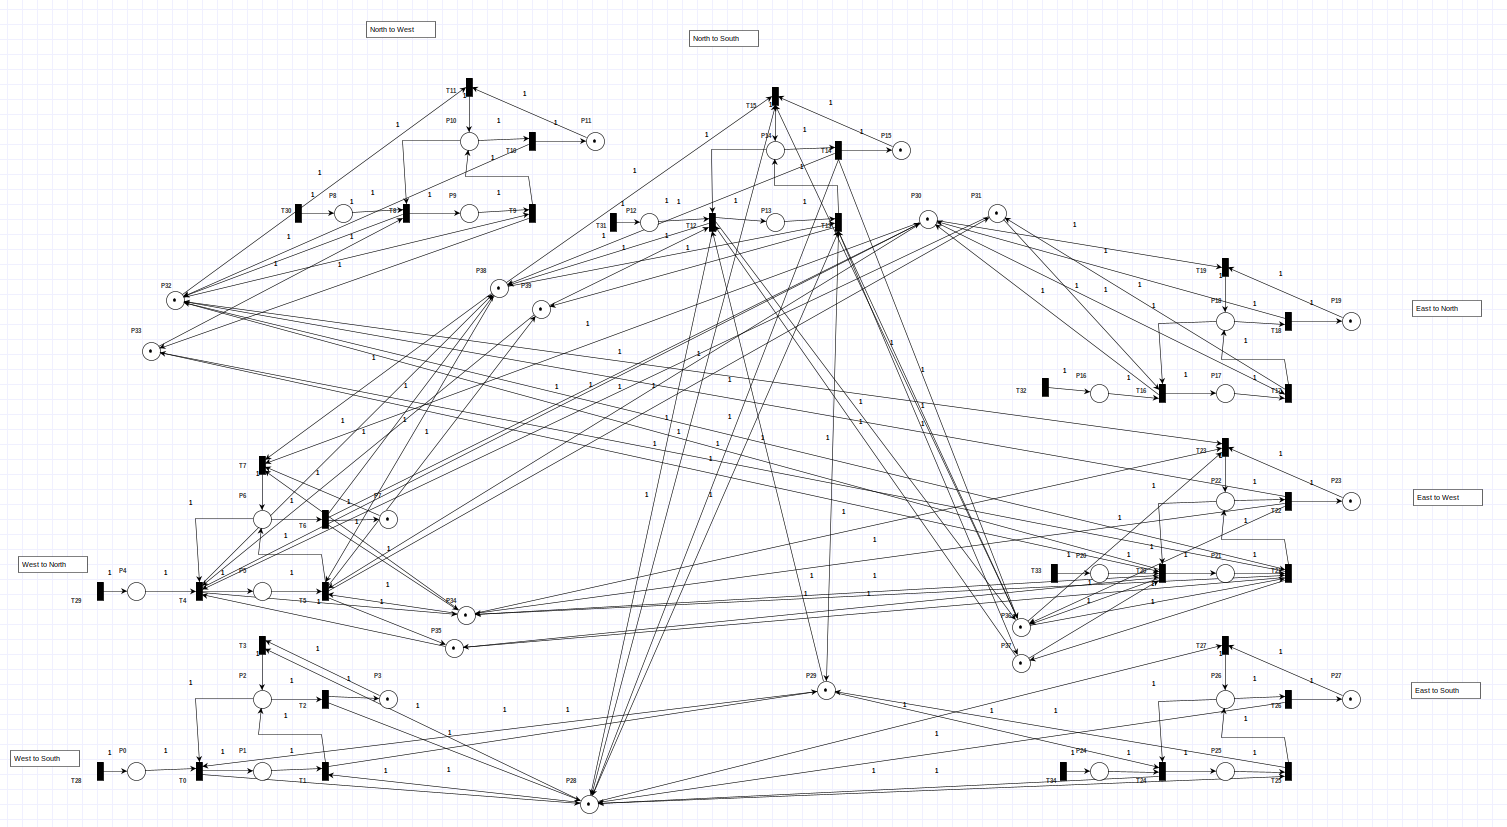
\includegraphics[width=1.0\textwidth]{figure/project_screenshots/semafori_finale_2.png}
    \caption{Modello finale con controlli}
    \label{fig:semafori_finale_monitor}
\end{figure}
\newpage


\chapter{Studio del Sistema}
\label{cap:cap4}
\lhead{\textbf{\rightmark}}
In questo capitolo viene condotta un'analisi del sistema. Si procede al calcolo della matrice di incidenza, alle GMEC, al calcolo dei posti monitor e alla marcatura iniziale di ogni posto monitor.
\newpage

\section{Matrici di incidenza}
\label{sec:4.1}
Al fine di compiere uno studio efficace del sistema, è innanzitutto necessario calcolare i suoi componenti fondamentali, quali la matrice di incidenza e la marcatura iniziale. Per tale calcolo si utilizza il sistema prima di implementare i controlli in modo da analizzare il sistema in uno stato iniziale.

Come descritto dalla formula \ref{eq:incidence_matrix}, la matrice di incidenza è definita come la differenza tra la matrice di post-incidenza e la matrice di pre-incidenza. Dunque, per poter calcolare la matrice di incidenza, è necessario calcolare le matrici di pre e post-incidenza:

\begin{table}[h!]
    \centering
    \resizebox{\textwidth}{!}{  % Resize the table to fit within the text width
    \begin{tabular}{|c|*{28}{c|}}
        \hline
        \rowcolor{lightgray}
        & T0 & T1 & T2 & T3 & T4 & T5 & T6 & T7 & T8 & T9 & T10 & T11 & T12 & T13 & T14 & T15 & T16 & T17 & T18 & T19 & T20 & T21 & T22 & T23 & T24 & T25 & T26 & T27 \\
        \hline
        P0 & 1 & 0 & 0 & 0 & 0 & 0 & 0 & 0 & 0 & 0 & 0 & 0 & 0 & 0 & 0 & 0 & 0 & 0 & 0 & 0 & 0 & 0 & 0 & 0 & 0 & 0 & 0 & 0 \\
        \hline
        P1 & 0 & 1 & 0 & 0 & 0 & 0 & 0 & 0 & 0 & 0 & 0 & 0 & 0 & 0 & 0 & 0 & 0 & 0 & 0 & 0 & 0 & 0 & 0 & 0 & 0 & 0 & 0 & 0 \\
        \hline
        P2 & 1 & 0 & 1 & 0 & 0 & 0 & 0 & 0 & 0 & 0 & 0 & 0 & 0 & 0 & 0 & 0 & 0 & 0 & 0 & 0 & 0 & 0 & 0 & 0 & 0 & 0 & 0 & 0 \\
        \hline
        P3 & 0 & 0 & 0 & 1 & 0 & 0 & 0 & 0 & 0 & 0 & 0 & 0 & 0 & 0 & 0 & 0 & 0 & 0 & 0 & 0 & 0 & 0 & 0 & 0 & 0 & 0 & 0 & 0 \\
        \hline
        P4 & 0 & 0 & 0 & 0 & 1 & 0 & 0 & 0 & 0 & 0 & 0 & 0 & 0 & 0 & 0 & 0 & 0 & 0 & 0 & 0 & 0 & 0 & 0 & 0 & 0 & 0 & 0 & 0 \\
        \hline
        P5 & 0 & 0 & 0 & 0 & 0 & 1 & 0 & 0 & 0 & 0 & 0 & 0 & 0 & 0 & 0 & 0 & 0 & 0 & 0 & 0 & 0 & 0 & 0 & 0 & 0 & 0 & 0 & 0 \\
        \hline
        P6 & 0 & 0 & 0 & 0 & 1 & 0 & 1 & 0 & 0 & 0 & 0 & 0 & 0 & 0 & 0 & 0 & 0 & 0 & 0 & 0 & 0 & 0 & 0 & 0 & 0 & 0 & 0 & 0 \\
        \hline
        P7 & 0 & 0 & 0 & 0 & 0 & 0 & 0 & 1 & 0 & 0 & 0 & 0 & 0 & 0 & 0 & 0 & 0 & 0 & 0 & 0 & 0 & 0 & 0 & 0 & 0 & 0 & 0 & 0 \\
        \hline
        P8 & 0 & 0 & 0 & 0 & 0 & 0 & 0 & 0 & 1 & 0 & 0 & 0 & 0 & 0 & 0 & 0 & 0 & 0 & 0 & 0 & 0 & 0 & 0 & 0 & 0 & 0 & 0 & 0 \\
        \hline
        P9 & 0 & 0 & 0 & 0 & 0 & 0 & 0 & 0 & 0 & 1 & 0 & 0 & 0 & 0 & 0 & 0 & 0 & 0 & 0 & 0 & 0 & 0 & 0 & 0 & 0 & 0 & 0 & 0 \\
        \hline
        P10 & 0 & 0 & 0 & 0 & 0 & 0 & 0 & 0 & 1 & 0 & 1 & 0 & 0 & 0 & 0 & 0 & 0 & 0 & 0 & 0 & 0 & 0 & 0 & 0 & 0 & 0 & 0 & 0 \\
        \hline
        P11 & 0 & 0 & 0 & 0 & 0 & 0 & 0 & 0 & 0 & 0 & 0 & 1 & 0 & 0 & 0 & 0 & 0 & 0 & 0 & 0 & 0 & 0 & 0 & 0 & 0 & 0 & 0 & 0 \\
        \hline
        P12 & 0 & 0 & 0 & 0 & 0 & 0 & 0 & 0 & 0 & 0 & 0 & 0 & 1 & 0 & 0 & 0 & 0 & 0 & 0 & 0 & 0 & 0 & 0 & 0 & 0 & 0 & 0 & 0 \\
        \hline
        P13 & 0 & 0 & 0 & 0 & 0 & 0 & 0 & 0 & 0 & 0 & 0 & 0 & 0 & 1 & 0 & 0 & 0 & 0 & 0 & 0 & 0 & 0 & 0 & 0 & 0 & 0 & 0 & 0 \\
        \hline
        P14 & 0 & 0 & 0 & 0 & 0 & 0 & 0 & 0 & 0 & 0 & 0 & 0 & 1 & 0 & 1 & 0 & 0 & 0 & 0 & 0 & 0 & 0 & 0 & 0 & 0 & 0 & 0 & 0 \\
        \hline
        P15 & 0 & 0 & 0 & 0 & 0 & 0 & 0 & 0 & 0 & 0 & 0 & 0 & 0 & 0 & 0 & 1 & 0 & 0 & 0 & 0 & 0 & 0 & 0 & 0 & 0 & 0 & 0 & 0 \\
        \hline
        P16 & 0 & 0 & 0 & 0 & 0 & 0 & 0 & 0 & 0 & 0 & 0 & 0 & 0 & 0 & 0 & 0 & 1 & 0 & 0 & 0 & 0 & 0 & 0 & 0 & 0 & 0 & 0 & 0 \\
        \hline
        P17 & 0 & 0 & 0 & 0 & 0 & 0 & 0 & 0 & 0 & 0 & 0 & 0 & 0 & 0 & 0 & 0 & 0 & 1 & 0 & 0 & 0 & 0 & 0 & 0 & 0 & 0 & 0 & 0 \\
        \hline
        P18 & 0 & 0 & 0 & 0 & 0 & 0 & 0 & 0 & 0 & 0 & 0 & 0 & 0 & 0 & 0 & 0 & 1 & 0 & 1 & 0 & 0 & 0 & 0 & 0 & 0 & 0 & 0 & 0 \\
        \hline
        P19 & 0 & 0 & 0 & 0 & 0 & 0 & 0 & 0 & 0 & 0 & 0 & 0 & 0 & 0 & 0 & 0 & 0 & 0 & 0 & 1 & 0 & 0 & 0 & 0 & 0 & 0 & 0 & 0 \\
        \hline
        P20 & 0 & 0 & 0 & 0 & 0 & 0 & 0 & 0 & 0 & 0 & 0 & 0 & 0 & 0 & 0 & 0 & 0 & 0 & 0 & 0 & 1 & 0 & 0 & 0 & 0 & 0 & 0 & 0 \\
        \hline
        P21 & 0 & 0 & 0 & 0 & 0 & 0 & 0 & 0 & 0 & 0 & 0 & 0 & 0 & 0 & 0 & 0 & 0 & 0 & 0 & 0 & 0 & 1 & 0 & 0 & 0 & 0 & 0 & 0 \\
        \hline
        P22 & 0 & 0 & 0 & 0 & 0 & 0 & 0 & 0 & 0 & 0 & 0 & 0 & 0 & 0 & 0 & 0 & 0 & 0 & 0 & 0 & 1 & 0 & 1 & 0 & 0 & 0 & 0 & 0 \\
        \hline
        P23 & 0 & 0 & 0 & 0 & 0 & 0 & 0 & 0 & 0 & 0 & 0 & 0 & 0 & 0 & 0 & 0 & 0 & 0 & 0 & 0 & 0 & 0 & 0 & 1 & 0 & 0 & 0 & 0 \\
        \hline
        P24 & 0 & 0 & 0 & 0 & 0 & 0 & 0 & 0 & 0 & 0 & 0 & 0 & 0 & 0 & 0 & 0 & 0 & 0 & 0 & 0 & 0 & 0 & 0 & 0 & 1 & 0 & 0 & 0 \\
        \hline
        P25 & 0 & 0 & 0 & 0 & 0 & 0 & 0 & 0 & 0 & 0 & 0 & 0 & 0 & 0 & 0 & 0 & 0 & 0 & 0 & 0 & 0 & 0 & 0 & 0 & 0 & 1 & 0 & 0 \\
        \hline
        P26 & 0 & 0 & 0 & 0 & 0 & 0 & 0 & 0 & 0 & 0 & 0 & 0 & 0 & 0 & 0 & 0 & 0 & 0 & 0 & 0 & 0 & 0 & 0 & 0 & 1 & 0 & 1 & 0 \\
        \hline
        P27 & 0 & 0 & 0 & 0 & 0 & 0 & 0 & 0 & 0 & 0 & 0 & 0 & 0 & 0 & 0 & 0 & 0 & 0 & 0 & 0 & 0 & 0 & 0 & 0 & 0 & 0 & 0 & 1 \\
        \hline
    \end{tabular}
    }
    \caption{Matrice di pre-incidenza}
    \label{tab:pre_incidence_matrix}
    
\end{table}
\newpage

\section{GMEC e supervisori}
\label{sec:4.2}
Dopo aver calcolato le matrici che caratterizzano il sistema semaforico di base, si procede a imporre dei vincoli per evitare che si creino situazioni pericolose o non desiderate. In particolare, si vuole evitare che i seguenti attraversamenti avvengano in contemporanea:

\begin{itemize}
    \item Da Est a Sud, da Ovest a Sud e da Nord a Sud;
    \item Da Ovest a Nord e da Est a Nord;
    \item Da Est a Ovest e da Nord a Ovest;
    \item Da Ovest a Nord e da Est a Ovest;
    \item Da Nord a Sud e da Est a Ovest;
    \item Da Ovest a Nord e da Nord a Sud.
    
\end{itemize}

Qualsiasi altra combinazione in contemporanea è consentita. Le combinazioni appena elencate sono vietate in quanto le prime tre prevedono il passaggio di veicoli provenienti da direzioni diverse e diretti verso la medesima direzione, creando un punto di conflitto in prossimità della direzione di arrivo. Le altre tre combinazioni, invece, sono vietate perchè vedono in contemporanea il passaggio di più veicoli provenienti da direzioni diverse ma che devono attraversare il centro dell'incrocio, generando così un altro punto di conflitto. Per implementare ciò, sono stati imposti i seguenti vincoli:

\begin{itemize}
    \item $M_{2} + M_{14} + M_{26} \leq 1$
    \item $M_{1} + M_{13} + M_{25} \leq 1$
    \item $M_{6} + M_{18} \leq 1$
    \item $M_{5} + M_{17} \leq 1$
    \item $M_{10} + M_{22} \leq 1$
    \item $M_{9} + M_{21} \leq 1$
    \item $M_{6} + M_{22} \leq 1$
    \item $M_{5} + M_{21} \leq 1$
    \item $M_{14} + M_{22} \leq 1$
    \item $M_{13} + M_{21} \leq 1$
    \item $M_{6} + M_{14} \leq 1$
    \item $M_{5} + M_{13} \leq 1$
\end{itemize}

Dopo aver delineato le GMEC, è possibile scriverle in forma matriciale per poi andare a calcolare le posizioni dei supervisori. Otteniamo quindi la matrice descritta nella tabella \ref{tab:w_matrix}:

\begin{table}[ht]
    \centering
    \resizebox{\textwidth}{!}{
        \begin{tabular}{|c|*{28}{c|}}
            \hline
            \rowcolor{lightgray}
            & T0 & T1 & T2 & T3 & T4 & T5 & T6 & T7 & T8 & T9 & T10 & T11 & T12 & T13 & T14 & T15 & T16 & T17 & T18 & T19 & T20 & T21 & T22 & T23 & T24 & T25 & T26 & T27 \\
            \hline
            w1 & 0 & 0 & 1 & 0 & 0 & 0 & 0 & 0 & 0 & 0 & 0 & 0 & 0 & 0 & 1 & 0 & 0 & 0 & 0 & 0 & 0 & 0 & 0 & 0 & 0 & 0 & 1 & 0 \\
            \hline
            w2 & 0 & 1 & 0 & 0 & 0 & 0 & 0 & 0 & 0 & 0 & 0 & 0 & 0 & 1 & 0 & 0 & 0 & 0 & 0 & 0 & 0 & 0 & 0 & 0 & 0 & 1 & 0 & 0 \\
            \hline
            w3 & 0 & 0 & 0 & 0 & 0 & 0 & 1 & 0 & 0 & 0 & 0 & 0 & 0 & 0 & 0 & 0 & 0 & 0 & 1 & 0 & 0 & 0 & 0 & 0 & 0 & 0 & 0 & 0 \\
            \hline
            w4 & 0 & 0 & 0 & 0 & 0 & 1 & 0 & 0 & 0 & 0 & 0 & 0 & 0 & 0 & 0 & 0 & 0 & 1 & 0 & 0 & 0 & 0 & 0 & 0 & 0 & 0 & 0 & 0 \\
            \hline
            w5 & 0 & 0 & 0 & 0 & 0 & 0 & 0 & 0 & 0 & 0 & 1 & 0 & 0 & 0 & 0 & 0 & 0 & 0 & 0 & 0 & 0 & 0 & 1 & 0 & 0 & 0 & 0 & 0 \\
            \hline
            w6 & 0 & 0 & 0 & 0 & 0 & 0 & 0 & 0 & 0 & 1 & 0 & 0 & 0 & 0 & 0 & 0 & 0 & 0 & 0 & 0 & 0 & 1 & 0 & 0 & 0 & 0 & 0 & 0 \\
            \hline
            w7 & 0 & 0 & 0 & 0 & 0 & 0 & 1 & 0 & 0 & 0 & 0 & 0 & 0 & 0 & 0 & 0 & 0 & 0 & 0 & 0 & 0 & 0 & 1 & 0 & 0 & 0 & 0 & 0 \\
            \hline
            w8 & 0 & 0 & 0 & 0 & 0 & 1 & 0 & 0 & 0 & 0 & 0 & 0 & 0 & 0 & 0 & 0 & 0 & 0 & 0 & 0 & 0 & 1 & 0 & 0 & 0 & 0 & 0 & 0 \\
            \hline
            w9 & 0 & 0 & 0 & 0 & 0 & 0 & 0 & 0 & 0 & 0 & 0 & 0 & 0 & 0 & 1 & 0 & 0 & 0 & 0 & 0 & 0 & 0 & 1 & 0 & 0 & 0 & 0 & 0 \\
            \hline
            w10 & 0 & 0 & 0 & 0 & 0 & 0 & 0 & 0 & 0 & 0 & 0 & 0 & 0 & 1 & 0 & 0 & 0 & 0 & 0 & 0 & 0 & 1 & 0 & 0 & 0 & 0 & 0 & 0 \\
            \hline
            w11 & 0 & 0 & 0 & 0 & 0 & 0 & 1 & 0 & 0 & 0 & 0 & 0 & 0 & 0 & 1 & 0 & 0 & 0 & 0 & 0 & 0 & 0 & 0 & 0 & 0 & 0 & 0 & 0 \\
            \hline
            w12 & 0 & 0 & 0 & 0 & 0 & 1 & 0 & 0 & 0 & 0 & 0 & 0 & 0 & 1 & 0 & 0 & 0 & 0 & 0 & 0 & 0 & 0 & 0 & 0 & 0 & 0 & 0 & 0 \\
            \hline
        \end{tabular}
    }
    \caption{Matrice W}
    \label{tab:w_matrix}
\end{table}

Utilizzando quindi la formula \ref{eq:gmec_vect}, possiamo quindi calcolare le righe da aggiungere alla matrice di incidenza per indicare i nuovi posti monitor:

\begin{table}[ht]
    \centering
    \resizebox{\textwidth}{!}{
        \begin{tabular}{|c|*{28}{c|}}
            \hline
            \rowcolor{lightgray}
            & T0 & T1 & T2 & T3 & T4 & T5 & T6 & T7 & T8 & T9 & T10 & T11 & T12 & T13 & T14 & T15 & T16 & T17 & T18 & T19 & T20 & T21 & T22 & T23 & T24 & T25 & T26 & T27 \\
            \hline
            P28 & 1 & -1 & 1 & -1 & 0 & 0 & 0 & 0 & 0 & 0 & 0 & 0 & 1 & -1 & 1 & -1 & 0 & 0 & 0 & 0 & 0 & 0 & 0 & 0 & 1 & -1 & 1 & -1 \\
            \hline
            P29 & -1 & 1 & 0 & 0 & 0 & 0 & 0 & 0 & 0 & 0 & 0 & 0 & -1 & 1 & 0 & 0 & 0 & 0 & 0 & 0 & 0 & 0 & 0 & 0 & -1 & 1 & 0 & 0 \\
            \hline
            P30 & 0 & 0 & 0 & 0 & 1 & -1 & 1 & -1 & 0 & 0 & 0 & 0 & 0 & 0 & 0 & 0 & 1 & -1 & 1 & -1 & 0 & 0 & 0 & 0 & 0 & 0 & 0 & 0 \\
            \hline
            P31 & 0 & 0 & 0 & 0 & -1 & 1 & 0 & 0 & 0 & 0 & 0 & 0 & 0 & 0 & 0 & 0 & -1 & 1 & 0 & 0 & 0 & 0 & 0 & 0 & 0 & 0 & 0 & 0 \\
            \hline
            P32 & 0 & 0 & 0 & 0 & 0 & 0 & 0 & 0 & 1 & -1 & 1 & -1 & 0 & 0 & 0 & 0 & 0 & 0 & 0 & 0 & 1 & -1 & 1 & -1 & 0 & 0 & 0 & 0 \\
            \hline
            P33 & 0 & 0 & 0 & 0 & 0 & 0 & 0 & 0 & -1 & 1 & 0 & 0 & 0 & 0 & 0 & 0 & 0 & 0 & 0 & 0 & -1 & 1 & 0 & 0 & 0 & 0 & 0 & 0 \\
            \hline
            P34 & 0 & 0 & 0 & 0 & 1 & -1 & 1 & -1 & 0 & 0 & 0 & 0 & 0 & 0 & 0 & 0 & 0 & 0 & 0 & 0 & 1 & -1 & 1 & -1 & 0 & 0 & 0 & 0 \\
            \hline
            P35 & 0 & 0 & 0 & 0 & -1 & 1 & 0 & 0 & 0 & 0 & 0 & 0 & 0 & 0 & 0 & 0 & 0 & 0 & 0 & 0 & -1 & 1 & 0 & 0 & 0 & 0 & 0 & 0 \\
            \hline
            P36 & 0 & 0 & 0 & 0 & 0 & 0 & 0 & 0 & 0 & 0 & 0 & 0 & 1 & -1 & 1 & -1 & 0 & 0 & 0 & 0 & 1 & -1 & 1 & -1 & 0 & 0 & 0 & 0 \\
            \hline
            P37 & 0 & 0 & 0 & 0 & 0 & 0 & 0 & 0 & 0 & 0 & 0 & 0 & -1 & 1 & 0 & 0 & 0 & 0 & 0 & 0 & -1 & 1 & 0 & 0 & 0 & 0 & 0 & 0 \\
            \hline
            P38 & 0 & 0 & 0 & 0 & 1 & -1 & 1 & -1 & 0 & 0 & 0 & 0 & 1 & -1 & 1 & -1 & 0 & 0 & 0 & 0 & 0 & 0 & 0 & 0 & 0 & 0 & 0 & 0 \\
            \hline
            P39 & 0 & 0 & 0 & 0 & -1 & 1 & 0 & 0 & 0 & 0 & 0 & 0 & -1 & 1 & 0 & 0 & 0 & 0 & 0 & 0 & 0 & 0 & 0 & 0 & 0 & 0 & 0 & 0 \\
            \hline
        \end{tabular}
    }
    \caption{Matrice di incidenza con i posti monitor}
    \label{tab:inc_matrix}
\end{table}

Utilizzando poi la formula \ref{eq:gmec_init} è poi possibile calcolare la marcatura iniziale di tutti i posti monitor. Nel caso in esame, la marcatura di tutti i postimonitor è pari a 1.

\begin{figure}[H]
    \centering
    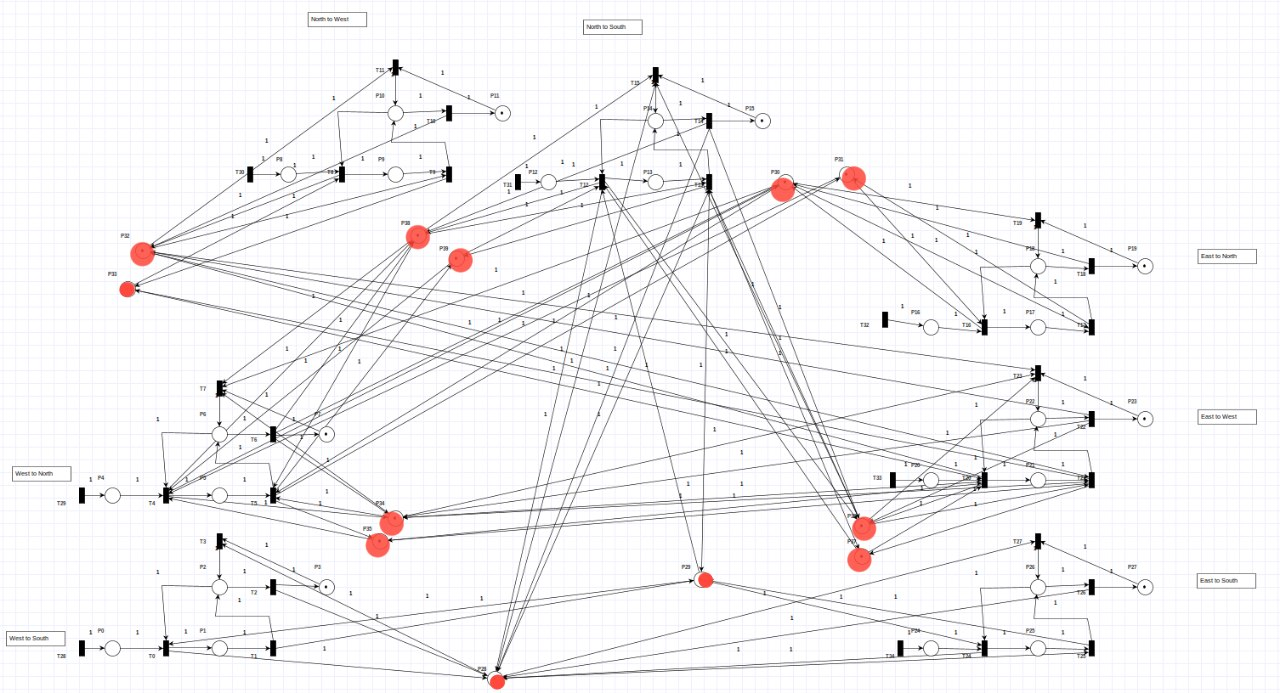
\includegraphics[width=1.0\textwidth]{figure/project_screenshots/sem_fin_controlli_evidenziati.jpg}
    \caption{Rete di Petri con i posti monitor evidenziati}
    \label{fig:petri_supervisori}
\end{figure}
\newpage


\backmatter

\nocite{*}

\end{document}
